% ============================================================
% Part 1 — Basic Worked Problems
% Topics: right-angled triangles, exact values, quadrant signs,
%         basic trigonometric identities, simple equations
% ============================================================

% ------------------------------------------------------------------
\begin{problem}[Graphing a Sine Function and its Phase Shift]

The graph of $y = \sin x$ (drawn in {\color{violet}purple}) is shown below
for $x \in [-2\pi,\, 2\pi]$.

\begin{center}
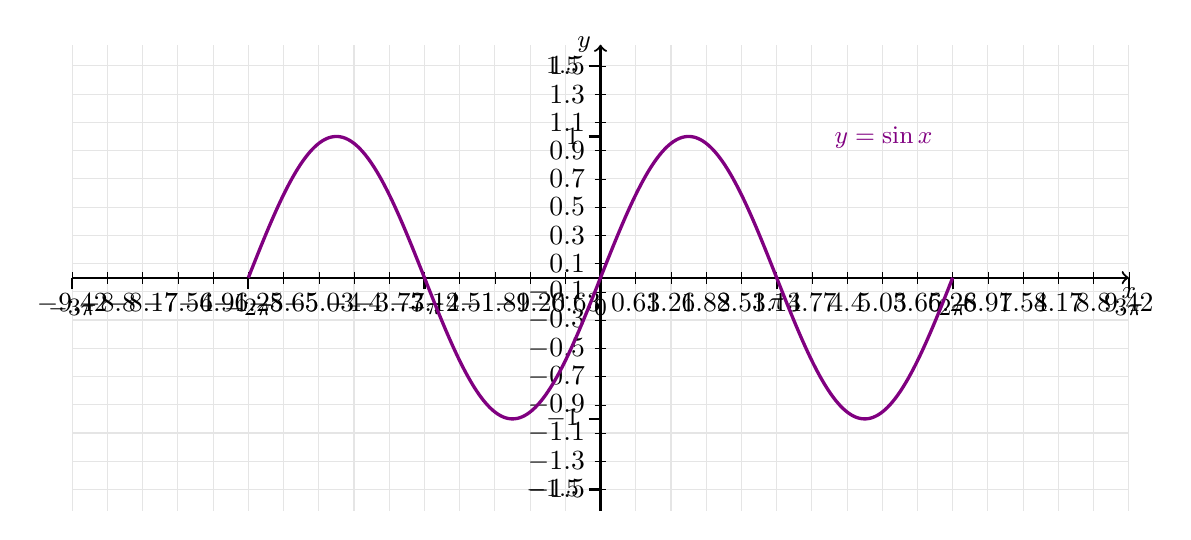
\begin{tikzpicture}
\begin{axis}[
    width=15cm, height=7.5cm,
    xmin=-9.4248, xmax=9.4248,
    ymin=-1.65,   ymax=1.65,
    % Fine grid: x at every pi/5, y at every 0.2
    xtick={-9.4248,-8.7965,...,9.4248},
    xticklabel={},
    ytick={-1.5,-1.3,...,1.5},
    yticklabel={},
    grid=major,
    grid style={gray!20, line width=0.4pt},
    % Axes through origin
    axis lines=center,
    axis line style={->, thick, black},
    % Labelled x ticks at multiples of pi
    extra x ticks={-9.4248,-6.2832,-3.1416,0,3.1416,6.2832,9.4248},
    extra x tick labels={$-3\pi$,$-2\pi$,$-\pi$,$0$,$\pi$,$2\pi$,$3\pi$},
    extra x tick style={
        tick align=outside,
        tick style={black, line width=0.8pt},
        grid=none,
        font=\small,
    },
    % Labelled y ticks
    extra y ticks={-1.5,-1,1,1.5},
    extra y tick labels={$-1.5$,$-1$,$1$,$1.5$},
    extra y tick style={
        tick align=outside,
        tick style={black, line width=0.8pt},
        grid=none,
        font=\small,
    },
    xlabel={$x$},
    ylabel={$y$},
    xlabel style={anchor=north, font=\small},
    ylabel style={anchor=east, font=\small},
    clip=false,
    tick style={black},
]
% y = sin(x) in purple over [-2pi, 2pi]
\addplot[violet, very thick, domain=-6.2832:6.2832, samples=400]
    {sin(deg(x))};
\node[violet, font=\small\itshape, above right]
    at (axis cs:4.0,0.85) {$y=\sin x$};
\end{axis}
\end{tikzpicture}
\end{center}

\medskip
On the axes below, draw the graph of
$\displaystyle y = \sin\!\left(x - \frac{\pi}{2}\right)$
for $x \in [-2\pi,\, 2\pi]$.

\begin{center}
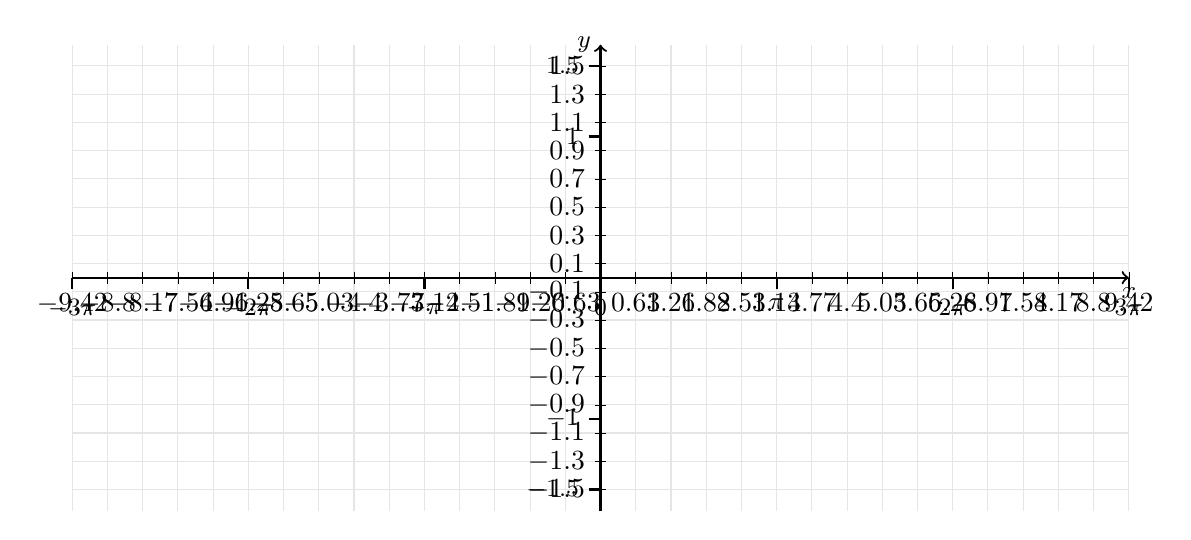
\begin{tikzpicture}
\begin{axis}[
    width=15cm, height=7.5cm,
    xmin=-9.4248, xmax=9.4248,
    ymin=-1.65,   ymax=1.65,
    xtick={-9.4248,-8.7965,...,9.4248},
    xticklabel={},
    ytick={-1.5,-1.3,...,1.5},
    yticklabel={},
    grid=major,
    grid style={gray!20, line width=0.4pt},
    axis lines=center,
    axis line style={->, thick, black},
    extra x ticks={-9.4248,-6.2832,-3.1416,0,3.1416,6.2832,9.4248},
    extra x tick labels={$-3\pi$,$-2\pi$,$-\pi$,$0$,$\pi$,$2\pi$,$3\pi$},
    extra x tick style={
        tick align=outside,
        tick style={black, line width=0.8pt},
        grid=none,
        font=\small,
    },
    extra y ticks={-1.5,-1,1,1.5},
    extra y tick labels={$-1.5$,$-1$,$1$,$1.5$},
    extra y tick style={
        tick align=outside,
        tick style={black, line width=0.8pt},
        grid=none,
        font=\small,
    },
    xlabel={$x$},
    ylabel={$y$},
    xlabel style={anchor=north, font=\small},
    ylabel style={anchor=east, font=\small},
    clip=false,
    tick style={black},
]
% Blank axes for student
\end{axis}
\end{tikzpicture}
\end{center}

\end{problem}
% ------------------------------------------------------------------

\begin{solution}

The graph of $y = \sin\!\left(x - \dfrac{\pi}{2}\right)$ is the graph of
$y = \sin x$ shifted \textbf{right} by $\dfrac{\pi}{2}$ (a phase shift of
$\dfrac{\pi}{2}$).

\medskip
Using the compound-angle identity:
\[
\sin\!\left(x - \frac{\pi}{2}\right)
  = \sin x\cos\frac{\pi}{2} - \cos x\sin\frac{\pi}{2}
  = \sin x \cdot 0 - \cos x \cdot 1
  = -\cos x.
\]
Hence $y = \sin\!\left(x - \dfrac{\pi}{2}\right) = -\cos x$.

\medskip
\textbf{Key points} on $[-2\pi,\, 2\pi]$:

\medskip
\begin{center}
\renewcommand{\arraystretch}{1.4}
\begin{tabular}{c|ccccccccc}
$x$ & $-2\pi$ & $-\dfrac{3\pi}{2}$ & $-\pi$ & $-\dfrac{\pi}{2}$
    & $0$    & $\dfrac{\pi}{2}$   & $\pi$  & $\dfrac{3\pi}{2}$
    & $2\pi$ \\[6pt] \hline
$y$ & $-1$ & $0$ & $1$ & $0$ & $-1$ & $0$ & $1$ & $0$ & $-1$
\end{tabular}
\end{center}

\medskip
The completed graph (curve shown in {\color{blue!70!black}blue}):

\begin{center}
\begin{tikzpicture}
\begin{axis}[
    width=15cm, height=7.5cm,
    xmin=-9.4248, xmax=9.4248,
    ymin=-1.65,   ymax=1.65,
    xtick={-9.4248,-8.7965,...,9.4248},
    xticklabel={},
    ytick={-1.5,-1.3,...,1.5},
    yticklabel={},
    grid=major,
    grid style={gray!20, line width=0.4pt},
    axis lines=center,
    axis line style={->, thick, black},
    extra x ticks={-9.4248,-6.2832,-3.1416,0,3.1416,6.2832,9.4248},
    extra x tick labels={$-3\pi$,$-2\pi$,$-\pi$,$0$,$\pi$,$2\pi$,$3\pi$},
    extra x tick style={
        tick align=outside,
        tick style={black, line width=0.8pt},
        grid=none,
        font=\small,
    },
    extra y ticks={-1.5,-1,1,1.5},
    extra y tick labels={$-1.5$,$-1$,$1$,$1.5$},
    extra y tick style={
        tick align=outside,
        tick style={black, line width=0.8pt},
        grid=none,
        font=\small,
    },
    xlabel={$x$},
    ylabel={$y$},
    xlabel style={anchor=north, font=\small},
    ylabel style={anchor=east, font=\small},
    clip=false,
    tick style={black},
]
% y = sin(x - pi/2) = -cos(x) in blue over [-2pi, 2pi]
\addplot[blue!70!black, very thick, domain=-6.2832:6.2832, samples=400]
    {-cos(deg(x))};
\node[blue!70!black, font=\small\itshape, above right]
    at (axis cs:3.5,0.85) {$y=\sin\!\left(x-\tfrac{\pi}{2}\right)$};
\end{axis}
\end{tikzpicture}
\end{center}

\end{solution}
% ------------------------------------------------------------------

\begin{takeaways}
\begin{itemize}[leftmargin=*]
  \item \textbf{Phase shift:} The graph of $y = \sin(x - c)$ for $c > 0$ is the
        graph of $y = \sin x$ shifted $c$ units to the \emph{right}.

  \item \textbf{Identity connection:}
        $\sin\!\left(x - \dfrac{\pi}{2}\right) = -\cos x$,
        so this curve is also the reflection of $y = \cos x$ in the $x$-axis.

  \item \textbf{Graphical check:} The shifted sine reaches its zeros at
        $x = \dfrac{\pi}{2} + k\pi$ ($k \in \mathbb{Z}$), its maximum of $1$
        at $x = \pi + 2k\pi$, and its minimum of $-1$ at $x = 2k\pi$
        — each exactly $\dfrac{\pi}{2}$ to the right of the corresponding
        feature on $y = \sin x$.
\end{itemize}
\end{takeaways}
